\chapter{Antecedentes}\label{ch:antecedentes}


\section{Antecedentes en los sistemas de componentes}
\label{sec:antecedentes-en-los-sistemas-de-componentes}

Los componentes son una parte \textbf{importante} de muchas aplicaciones
orientadas a los usuarios finales.
En esta sección se presentarán algunas aplicaciones que permiten
la instalación de componentes:

\begin{itemize}
    \item \textbf{Navegadores web}: los navegadores web
    son las principales aplicaciones con complementos.
    Programas como \textit{Firefox}\cite{FIREFOX} o
    \textit{Google Chrome}\cite{CHROME}
    presentan una \textbf{tienda} donde el usuario puede instalar
    componentes con un solo clic.
    Estos componentes suelen estar desarrollados en \textit{JavaScript}
    o \textit{TypeScript}.
    \item \textbf{Entornos de desarrollo integrados}: los entornos de
    desarrollo más conocidos también tienen la capacidad de expandir
    sus herramientas mediante componentes.
    Estos componentes pueden introducir desde pequeños cambios
    a \textbf{tecnologías completamente nuevas} a la aplicación, y suelen
    estar programados en el mismo lenguaje que el entorno de desarrollo.
    Ejemplos de entornos de desarrollo con componentes
    son \textit{IntelliJ IDEA}\cite{INTELLIJIDEA} y \textit{Eclipse}\cite{ECLIPSE},
    ambos con componentes desarrollados en \textit{Java}\cite{JAVA}.
    \item \textbf{Videojuegos}: existe una gran variedad
    de videojuegos con posibilidad de expansión mediante
    componentes, llamados \textit{\textbf{mods}} en este entorno.
    Las librerías que proporcionan soporte para \textit{mods}
    pueden estar desarrolladas por los jugadores o venir
    integradas en el juego base.
    Un ejemplo de librerías desarrolladas por jugadores es
    \textit{Spigot}\cite{SPIGOT} para \textit{Minecraft}, y un ejemplo
    de librerías integradas por los desarrolladores
    serían los videojuegos de \textit{Steam} con soporte
    para \textit{Steam Workshop}\cite{STEAM_WORKSHOP}.
    \item \textbf{Aplicaciones en la nube}: existen
    algunas aplicaciones en la nube que permiten
    al usuario complementar su experiencia con diversos
    componentes desarrollados por terceros.
    Es el caso de \textit{Google Drive}, el cual permite
    instalar componentes para la visualización y
    edición de archivos.
    Este enfoque de los componentes es muy interesante,
    ya que es el \textbf{proveedor de la aplicación} el que
    instala el componente y no el usuario.
\end{itemize}


\section{Antecedentes en el desarrollo para la consola \textit{NES}}
\label{sec:antecedentes-en-el-desarrollo-para-la-consola-nes}

Existe una gran cantidad de herramientas para poder desarrollar
una aplicación o videojuego para la consola \textit{NES}\cite{NES}.
Las principales son las \textbf{proporcionadas por \textit{Nintendo}}
en la década de los 80 a las desarrolladoras, pero estas
aplicaciones son muy antiguas y necesitan un kit de desarrollo
completo que solo \textit{Nintendo} puede proporcionar.
Las aplicaciones que se utilizan actualmente están
\textbf{desarrolladas por personas externas} a la compañía,
manteniendo vivo el desarrollo y uso de esta consola.

Estas herramientas resuelven problemas muy concretos
presentes en el desarrollo de videojuegos, y ninguna
de ellas puede considerarse un entorno de desarrollo integrado.
Algunas de estas herramientas son las siguientes:

\begin{itemize}
    \item \textbf{Nestopia}\cite{NESTOPIA}:
    \textit{Nestopia} es uno de los emuladores
    para la consola \textit{NES} más importantes.
    Desarrollado en \textit{C++}, \textit{Nestopia} tiene soporte
    para más de 200 controladores de memoria y gran cantidad de periféricos.
    \emph{Nestopia} está considerado uno de los emuladores más
    fieles que existen.
    \item \textbf{Asm6f}\cite{ASM6F}:
    ensamblador de código abierto
    para el código ensamblador 6052.
    \textit{Asm6f} permite ensamblar el código en
    \textbf{archivos \textit{INES 2.0}}
    que pueden utilizarse en emuladores, además
    de tener características especiales como soporte
    para instrucciones no oficiales.
    \item \textbf{NEXXT}: es una pequeña
    aplicacion que permite editar los gráficos de los
    videojuegos de la \textit{NES}.
    La aplicación cuenta con funciones para recrear escenas
    mediante los \textit{tilesets} creados.
\end{itemize}

En el desarrollo para la consola \textit{NES} también se utiliza
una serie de formatos de archivos comunes:

\begin{itemize}
    \item \textbf{Archivos \textit{PCX}}: \textit{PCX} es un formato de imagen desarrollado
    en el año 1985 que cuenta con una codificación \textit{run-length}.
    Actualmente, el formato ha caído en desuso, pero sus propiedades
    lo hacen un \textbf{gran candidato} para almacenar gráficos
    de la \textit{NES} antes de ser ensamblados.
    Esto se debe a su capacidad de codificar los colores mediante
    una \textit{paleta} de una manera sencilla.
    Al almacenar los valores de los píxeles como índices y no
    como colores, el formato \textit{PCX} se convierte en un
    candidato ideal para gráficos dependientes de una paleta
    externa, como es el caso de los gráficos de una \textit{NES}.
    \item \textbf{Archivos \textit{iNES}}: \textit{iNES}
    es el formato de archivo más utilizado
    para almacenar videojuegos para la consola \textit{NES}.
    Este formato comienza con una cabecera con los datos que suelen
    estar codificados en el propio cartucho, como puede ser el modo
    espejo, el controlador de memoria o la región.
    La cabecera también contiene el tamaño de la región del
    programa (\textit{PGR}) y la región de gráficos (\textit{CHR})
    que van detrás de ella.
\end{itemize}


\section{\textit{JAMS}: \textit{Just Another MIPS Simulator}}
\label{sec:jams-just-another-mips-simulator}

\textit{JAMS}\cite{JAMS} es un \textbf{entorno de desarrollo integrado} moderno especializado
en \textbf{lenguajes ensambladores} desarrollado en \textit{Java}\cite{JAVA}
con la librería \textit{JavaFX}\cite{JAVAFX}.
El entorno de desarrollo está enfocado en \textbf{proyectos},
con una estructura basada en pequeñas herramientas que pueden
desplegarse desde los laterales de la ventana principal.
La aplicación es totalmente personalizable, pudiendo el usuario
cambiar su idioma, su aspecto o su comportamiento desde
su configuración.

\begin{figure}[h]
    \centering
    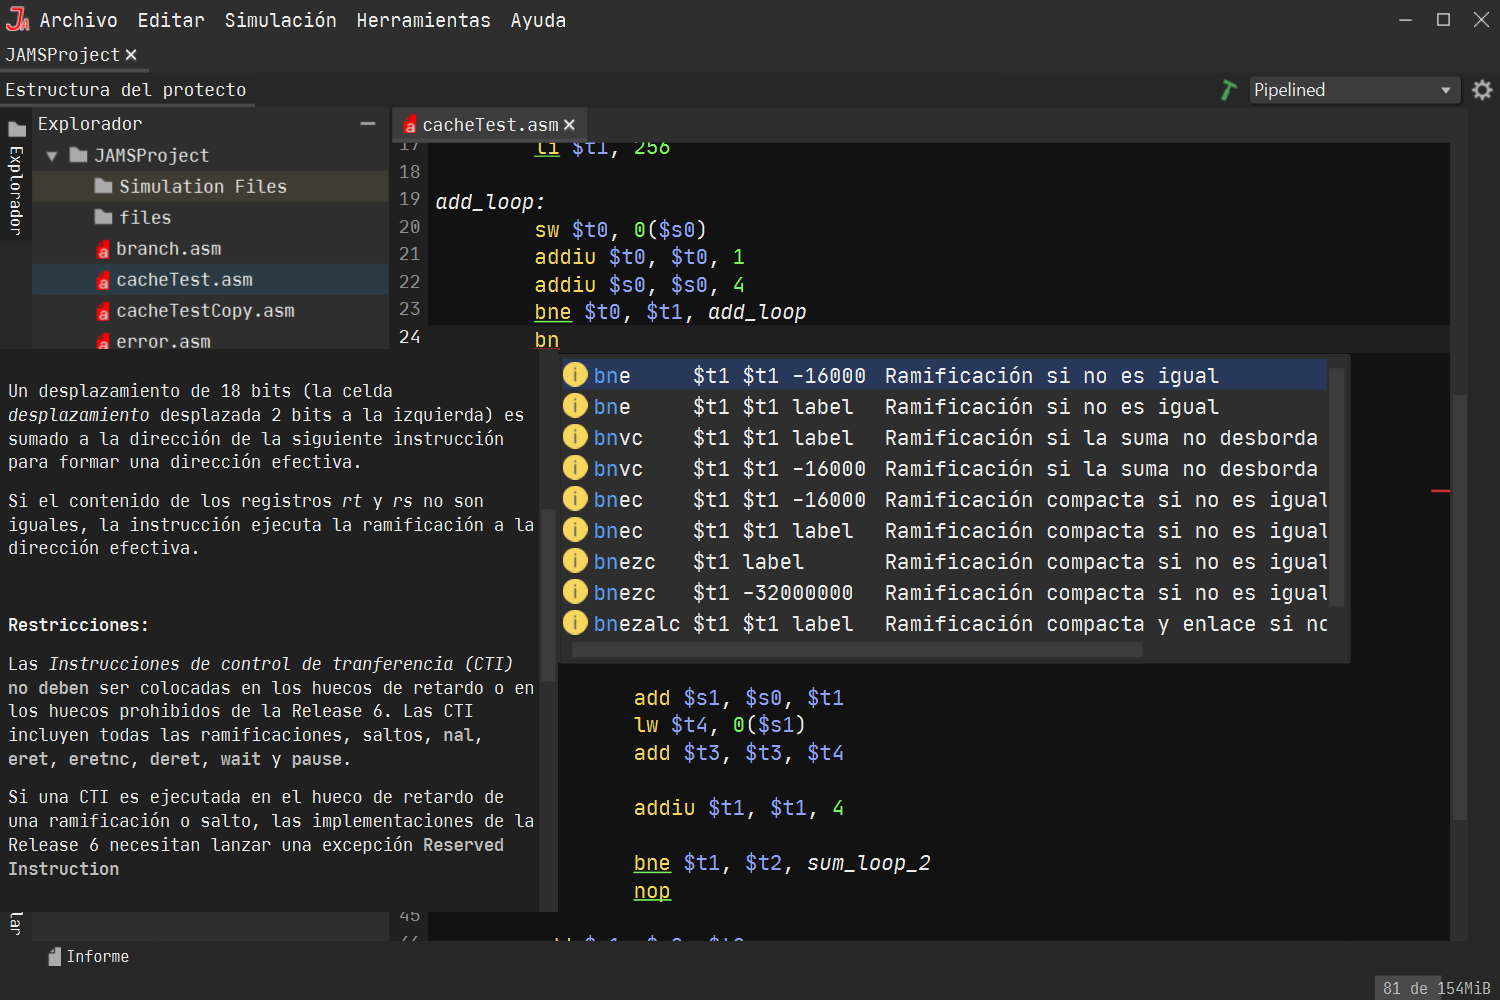
\includegraphics[width=0.8\textwidth]{images/antecedentes/jams-documentation}
    \caption{Entorno de desarrollo para \textit{MIPS32}}
    \label{fig:jams-documentation}
\end{figure}

Una de las características de \textit{JAMS} más importantes
para este Trabajo Fin de Grado es su alta modularidad.
\textit{JAMS} está diseñado teniendo en cuenta la posibilidad
de dar soporte a componentes en un futuro, facilitando los cambios
necesarios en el código.
Las herramientas usadas en el entorno de desarrollo para
\textit{MIPS32} (visible en la figura \ref{fig:jams-documentation})
suelen tener una estructura genérica,
lo que facilita su reutilización en el entorno de desarrollo
propuesto en este trabajo.